\section{User Interface}
The User interface section will over the actions that a user will be able to take, explaining all menus, buttons,
pull down menus, selections, etc. This section will also describe actions that system administrators will need to
take to start and stop the application.

\begin{figure}[H]
  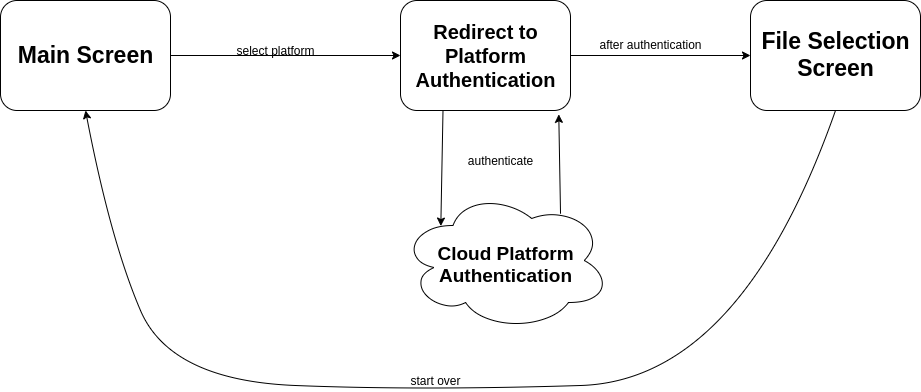
\includegraphics[scale=.5]{user_flow}
  \centering
  \caption{The workflow for the user}
\end{figure}

    \subsection{User Interaction}
    The user will interact with the application through the web interface. They will have several screens (views)
    to navigate through. Those will include the main screen to select the platform to download from (AWS, Dropbox,
    Google Drive, etc) and then will be presented with a view to enter their credentials. Once their credentials
    are entered they will be presented with the final view which contains their directory structure and contents
    and they will be able to multi-select which of those contents they would like to download.

    For more information, readers can refer to the \texttt{Prototype Screenshots for the Downloader Application}\cite{prot}
    which will cover the work flow for the user and screenshots of the preliminary screens.
    
      \subsubsection{Platform Selection Screen}
      The first page of the application that the user will come across is a page to select which platform they will be
      viewing and downloading files from. This page will contain a \textit{pull down} menu containing each of the
      cloud platforms that the application supports. Once the user has selected the one they want, they will press the
      \textit{submit} button which will bring them to the next page.

      \begin{figure}[H]
        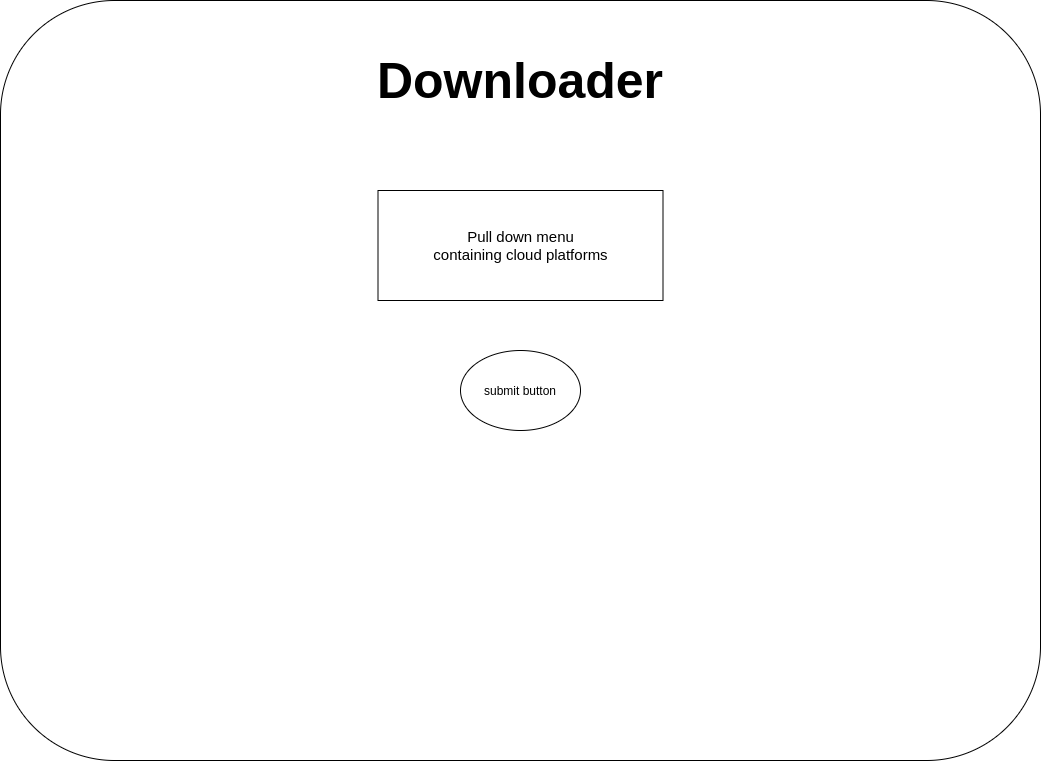
\includegraphics[scale=.5]{main_screen}
        \centering
        \caption{The first screen of the application.}
      \end{figure}

      \subsubsection{Authentication Screen}
      After the user has selected their platform from the \textit{platform selection screen}, the application will
      determine what kind of authorization information it needs from the user and prompt the user to enter this information.
      This will include a user name, and either a password, access token or both. Once the user enters their credentials for
      their cloud account they will press the \textit{ok} button to allow the application to authenticate to the cloud platform
      and read their files. They will be redirected to the final screen at this point.
    
      \subsubsection{File Selection Screen}
      On the final screen of the application, after the user has selected and authenticated to a cloud platform they will be
      presented with the files and directory structure that they have on that platform. The user will be able to navigate their
      directory structure from this screen as well as multi-select which files and directories they would like to download.

      Once the user is ready to download their files and directories they will click on the \textit{download} button which will
      initiate the downloading of their files to where the user's web browser directs downloads to. Once the download is complete
      the user can exit the browser window, select the \textit{start over} button to go back to the \textit{Platform Selection Screen}
      or select a different set of files to download.

      \begin{figure}[H]
        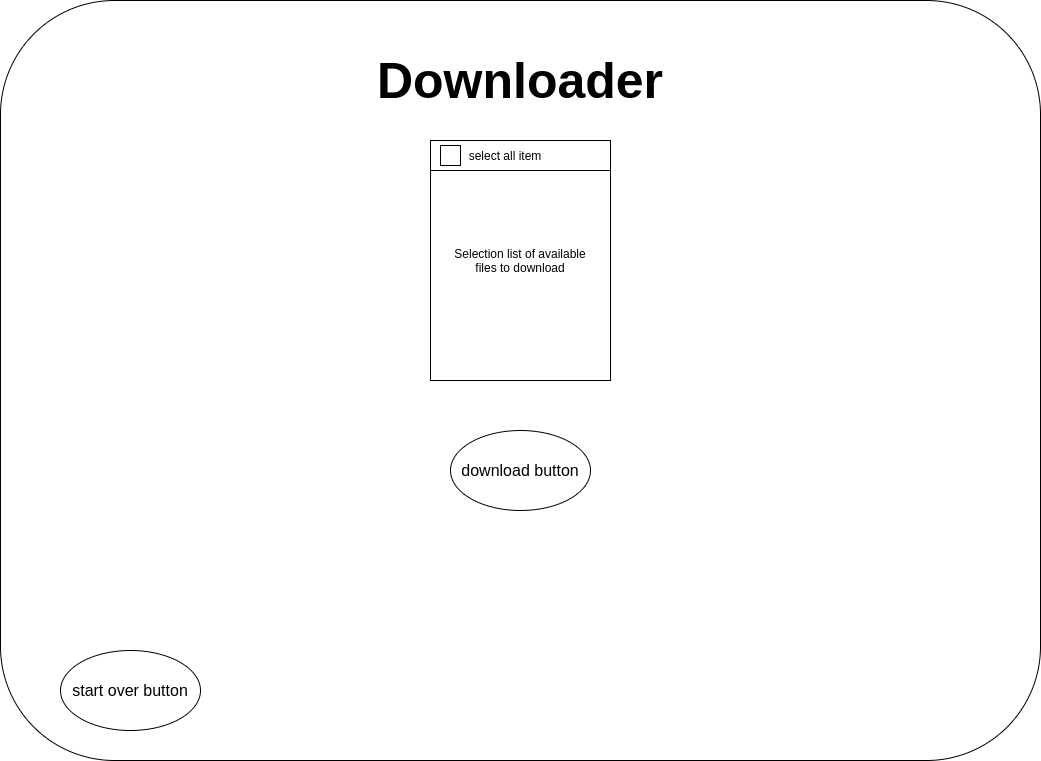
\includegraphics[scale=.5]{download_screen}
        \centering
        \caption{The screen to view and download files.}
      \end{figure}
    
    \subsection{Administrator Interaction}
    The system administrator will interact with the application by using the built-in Django commands on the
    server that the application will run on. They will mainly only be starting and stopping the web application
    through this interface. Django does have a built-in web administration page but this application will not
    need to take advantage of this functionality.

      \subsubsection{Start Application}
      To start the application the system administrator will use the Django created \textit{manage.py} file
      to invoke the application on its default port of \textit{8000}.
      \begin{verbatim}
      $ python manage.py runserver
      \end{verbatim}

      If the administrator would like to expose the webserver beyond \textit{localhost} and let other devices connect or
      use a different port then they will pass an argument with the sources and new port. For example, to let any source
      connect to the server from port \textit{8080} the administrator would type:
      \begin{verbatim}
      $ python manage.py runserver 0:8080
      \end{verbatim}
      The ``0'' before the \textit{colon} is shorthand for \textit{0.0.0.0} which will allow any source to connect.

      \subsubsection{Stop Application}
      Since the web server will be a foreground process in the terminal, the web administrator will press \textit{ctrl + c}
      to kill the process or any of the other ten thousand ways to terminate a process on a *nix system.


